%
% All data regarding this presentation has to be set in here
%
\title[TitleShort]{Eclipse IDE}
%\subtitle{SubTitle}
\author[AuthorShort]{Robert, Stefan, David}
\date[22.11.2016]{Meeting}
\pgfdeclareimage[height=3.0cm]{titlegraphic}{images/logoTitle}

\usepackage[utf8]{inputenc}

%
% Language style to use, either german or english
%

%German style
\usepackage[ngerman]{babel}
\newtranslation[to=ngerman]{Section}{Teil} 

%English style
%\usepackage[english]{babel}

%
% All included tex files / sections have to be declared here
%
\newcommand{\allSections}{
%\section{Section1}
%\subsection{Subsection1}
%\begin{frame}
%  \frametitle{FrameTitle1}
%  \framesubtitle{FrameSubtitle1}
%  Content:
%  \begin{itemize}
%  \item \texttt{slides.tex}: übersetzbares Dokument
%  \item \texttt{common.tex}: benutzerspezifische Pakete
%  \item \texttt{data.tex}: Inhalt der Präsentation
%  \item \texttt{lit.bib}: BIBTeX Datei für Literaturverzeichnis
%  \item \texttt{images}: Verzeichnis für Grafiken
%  \end{itemize}
%\end{frame}

\section{Integration in Eclipse}
\begin{frame}
  \frametitle{Integration in Eclipse}
  \begin{itemize}
    \item Plugins können an vordefinierten \textbf{Extension Points} die Funktionalität von Eclipse erweitern
  \end{itemize}
\end{frame}

\section{Struktur eines Plugins}
\begin{frame}
  \frametitle{Struktur eines Plugins}
  \begin{itemize}
  \item \texttt{plugin.xml}
  \item \texttt{MANIFEST.MF}
  \item Bibliotheken
  \item Implementierung
  \item Ressourcen (z.B. Icons)
  \end{itemize}
\end{frame}

\begin{frame}
  \frametitle{Struktur eines Plugins}
  \framesubtitle{plugin.xml}
  \begin{itemize}
  \item Definition der Extension Points, die vom Plugin erweitert werden
  \item Definition der Extension Points, die das Plugin bereitstellt, sodass andere Plugins diese erweitern können
  \item Struktur: \\
  \texttt{<plugin>\\ \ \ <extension point="...">\\ \ \ <...> (abhängig vom Extension Point)\\ \ \ </extension>\\ </plugin>}
  \end{itemize}
\end{frame}

\begin{frame}
  \frametitle{Struktur eines Plugins}
  \framesubtitle{MANIFEST.MF}
  \begin{itemize}
    \item OSGi Manifest
    \item Definition von Metadaten des Plugins
    \begin{itemize}
      \item Name, Version, Package
      \item Abhängigkeiten
    \end{itemize}
	\item \begin{minipage}{\linewidth}
		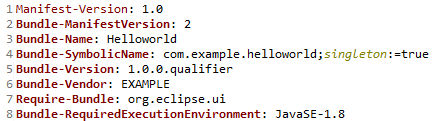
\includegraphics[scale=0.8]{images/manifest.png}
      \end{minipage}	 
  \end{itemize}
\end{frame}

\section{Architektur}
\begin{frame}
  \frametitle{Architektur}
  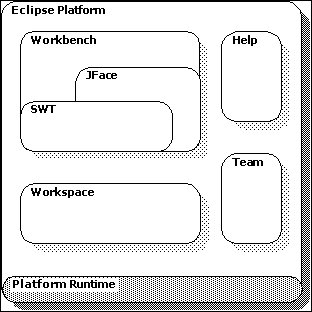
\includegraphics[scale=0.8]{images/architecture.jpg}
\end{frame}

\begin{frame}
  \frametitle{Architektur}
  \begin{itemize}
    \item Definiert Extension Points
    \item Basiert auf OSGi Framework
    \item Verwaltet installierte Plugins
    \item Aktiviert diese, wenn sie benötigt werden
  \end{itemize}
\end{frame}

\begin{frame}
  \frametitle{Architektur}
  \framesubtitle{Workspace}
  \begin{itemize}
    \item Definiert API, um Ressourcen zu erstellen und zu verwalten
    \item Ressourcen sind bspw.: Prjekte, Dateien, Ordner
    \item Werden im Dateisystem gespeichert
  \end{itemize}
\end{frame}

\begin{frame}
  \frametitle{Architektur}
  \framesubtitle{Workbench UI}
  \begin{itemize}
    \item Extension Points um UI Komponenten hinzuzufügen
    \item Toolkits \textbf{JFace} und \textbf{SWT} zur Erstellung von UIs
  \end{itemize}
\end{frame}

\begin{frame}
  \frametitle{Architektur}
  \framesubtitle{Help}
  \begin{itemize}
    \item Definiert Extension Points um Hilfe und Dokumentationen anzuzeigen
  \end{itemize}
\end{frame}

\begin{frame}
  \frametitle{Architektur}
  \framesubtitle{Team}
  \begin{itemize}
    \item Definiert Model für das Management und die Versionierung von Ressourcen
  \end{itemize}
\end{frame}

\begin{frame}
  \frametitle{Architektur}
  \framesubtitle{Debug}
  \begin{itemize}
    \item Definiert sprachunabhängiges Model zum Debugging und UI zum Erstellen von Debuggern
  \end{itemize}
\end{frame}

\begin{frame}
  \frametitle{Architektur}
  \framesubtitle{Utilities}
  \begin{itemize}
    \item Verschiedene andere Funktionalität:
    \begin{itemize}
      \item Suchen und Ersetzen
      \item XML Konfiguration
      \item Zugriff auf Server
    \end{itemize}
  \end{itemize}
\end{frame}

\section{Extension Points}
\begin{frame}
  \frametitle{Extension Points}
  \framesubtitle{Commands}
  \begin{itemize}
    \item Identifizierung durch ID
    \item Werden durch Menüs und Tastenkombinationen ausgeführt
    \item Definieren lediglich Verhalten
    \item Implementiert durch \textbf{Handler}
    \begin{itemize}
      \item verschiedene Plugins können dasselbe Command implementieren
    \end{itemize}
    \item \texttt{org.eclipse.ui.commands}
  \end{itemize}
\end{frame}

\begin{frame}
  \frametitle{Extension Points}
  \framesubtitle{Handler}
  \begin{itemize}
    \item Implementiert das Verhalten eines \textbf{Commands}
    \item Workbench entscheidet, welcher Handler ein Command behandelt
    \item \texttt{org.eclipse.ui.handlers}
  \end{itemize}
\end{frame}

\begin{frame}
  \frametitle{Extension Points}
  \framesubtitle{Key Binding}
  \begin{itemize}
    \item Assoziation zwischen Command und Tastenkombination
    \item Tastenkombinationen haben einen Kontext in dem sie aktiv sind
    \item \texttt{org.eclipse.ui.bindings}
  \end{itemize}
\end{frame}

\section{Workspace UI}
\begin{frame}
  \frametitle{Workspace UI}
  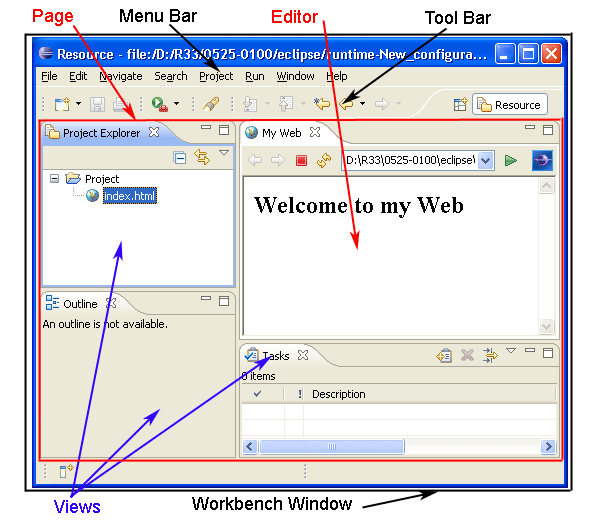
\includegraphics[scale=0.4]{images/workspace-ui.png}
\end{frame}

\begin{frame}
  \frametitle{Workspace UI}
  \framesubtitle{Seiten}
  \begin{itemize}
    \item Eine \textbf{Seite (Page)} kann veschiedene Komponenten enthalten
    \item Pages müssen typischerweise nicht programmiert werden
  \end{itemize}
\end{frame}

\begin{frame}
  \frametitle{Workspace UI}
  \framesubtitle{Perspektive}
  \begin{itemize}
    \item Eine \textbf{Perspektive} definiert eine der Aufgabe angemessene Menge von Views, deren Layout und ausführbare Aktionen
  \end{itemize}
\end{frame}

\begin{frame}
  \frametitle{Workspace UI}
  \framesubtitle{View}
  \begin{itemize}
    \item Eine \textbf{View} wird verwendet, um durch eine Informationshierarchie zu navigieren, Editoren zu öffnen oder Einstellungen des Editors zu bearbeiten
    \item \texttt{org.eclipse.ui.views}
  \end{itemize}
\end{frame}

\begin{frame}
  \frametitle{Workspace UI}
  \framesubtitle{Editor}
  \begin{itemize}
    \item Ein Editor wird verwendet, um ein Dokument oder ein anderes Objekt anzuzeigen und zu bearbeiten
    \item \texttt{org.eclipse.ui.editors}
  \end{itemize}
\end{frame}

\begin{frame}
  \frametitle{Workspace UI}
  \framesubtitle{Preferences}
  \begin{itemize}
    \item Plugins können Einträge zur Baumstruktur der Einstellungen hinzufügen
    \item \texttt{org.eclipse.ui.preferencePages}
  \end{itemize}
\end{frame}

\begin{frame}
  \frametitle{Workspace UI}
  \framesubtitle{Tool Bar und Menu Bar}
  \begin{itemize}
    \item \textbf{Menu Bar}: die globale Tool Bar von Eclipse
    \item Weitere Tool Bars und Kontextmenüs können erstellt werden
    \item Einträge führen \textbf{Commands} aus oder beinhalten weitere Menüs
    \item \texttt{org.eclipse.ui.menus}
  \end{itemize}
\end{frame}

\begin{frame}
  \frametitle{Workspace UI}
  \framesubtitle{Dialoge und Wizards}
  \begin{itemize}
    \item \textbf{Dialoge:}
    \begin{itemize}
      \item Anzeige von Meldungen (z.B. Fehlern)
      \item Bestätigung einer Aktion
      \item Eingabe von Werten
    \end{itemize}
    \item \textbf{Wizard:}
    \begin{itemize}
      \item Geführte Eingabe von Daten in einer Sequenz verschiedener Formulare (z.B. Erstellen eines Projekts)
      \item Besteht aus \textbf{Wizard Dialog} und mehreren \textbf{Wizard Pages}
      \item Vordefinierte Extension Points existieren für Wizards zum Erstellen, Importieren und Exportieren von Obk
    \end{itemize}
  \end{itemize}
\end{frame}



\begin{frame}
\frametitle{Literature}
\bibliography{lit}
\end{frame}


}